		\begin{frame}
			\frametitle{Pressure Ulcers}
			\begin{columns}[c]
				\column{0.45\textwidth}
				\begin{itemize}
					\item Pressure ulcers are secondary injuries
					\begin{itemize}
						\item People with reduced mobility
					\end{itemize}

					\item Skin breakdown due to moisture, shear / friction

					\item Categorized by NPUAP in stages
					\begin{itemize}
						\item From shallow to deep
					\end{itemize}
				\end{itemize}

				\column{0.55\textwidth}
					\begin{figure}
						\centering
						\subfloat{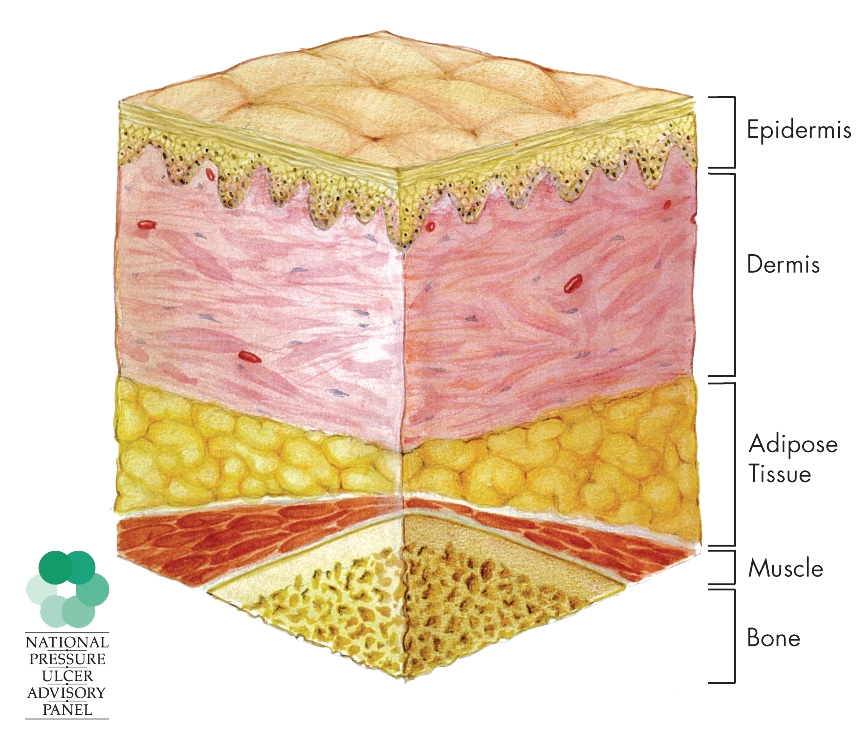
\includegraphics[width=0.33\textwidth]{assets/npuap/normal.png}}

						\subfloat{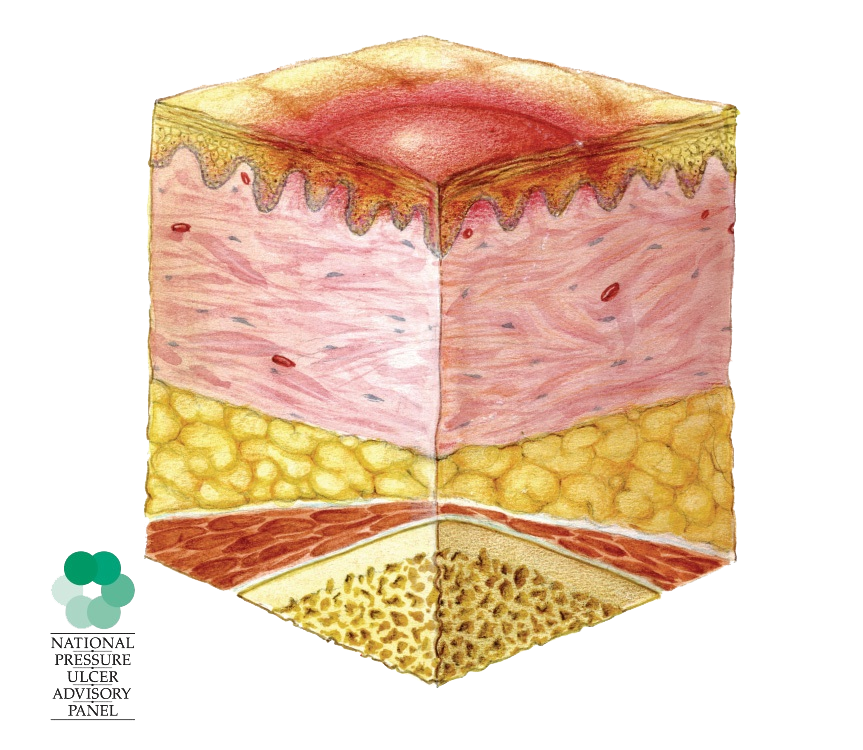
\includegraphics[width=0.33\textwidth]{assets/npuap/stage1.png}}
						\subfloat{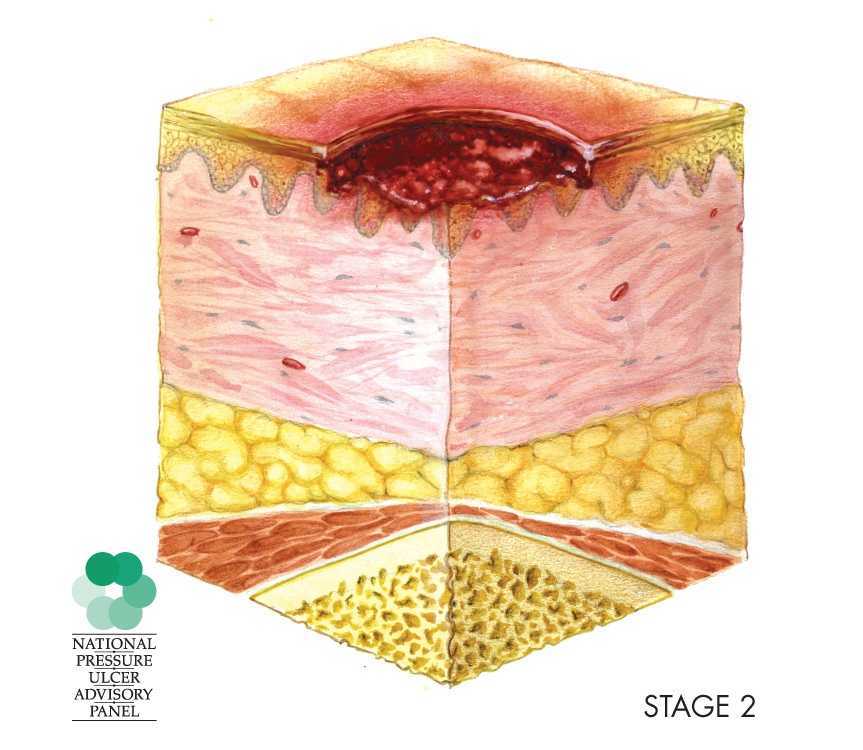
\includegraphics[width=0.33\textwidth]{../latex/assets/npuap/stage2.png}}
						\subfloat{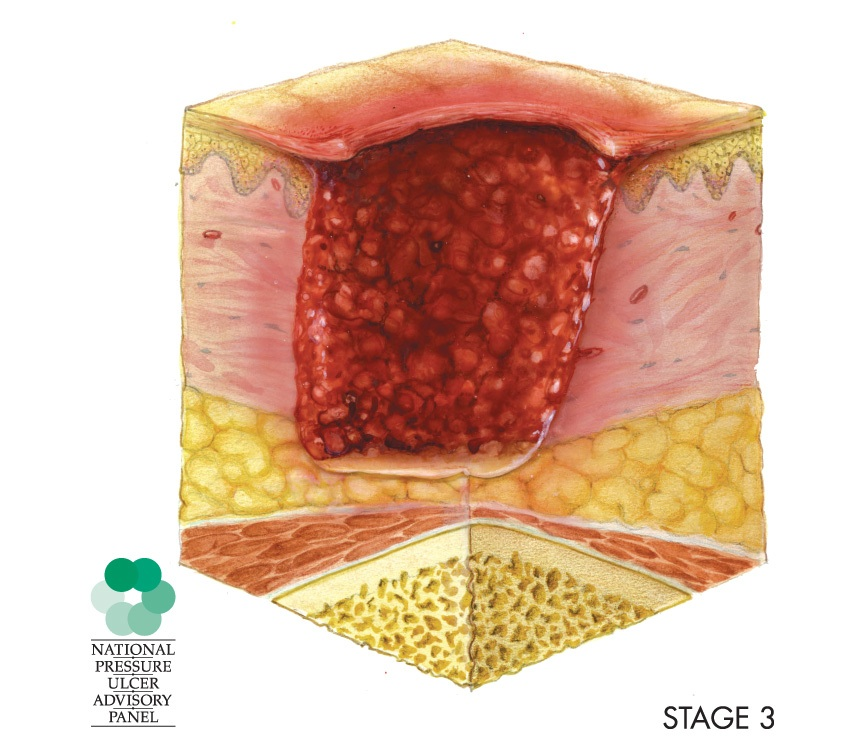
\includegraphics[width=0.33\textwidth]{../latex/assets/npuap/stage3.png}}

						\subfloat{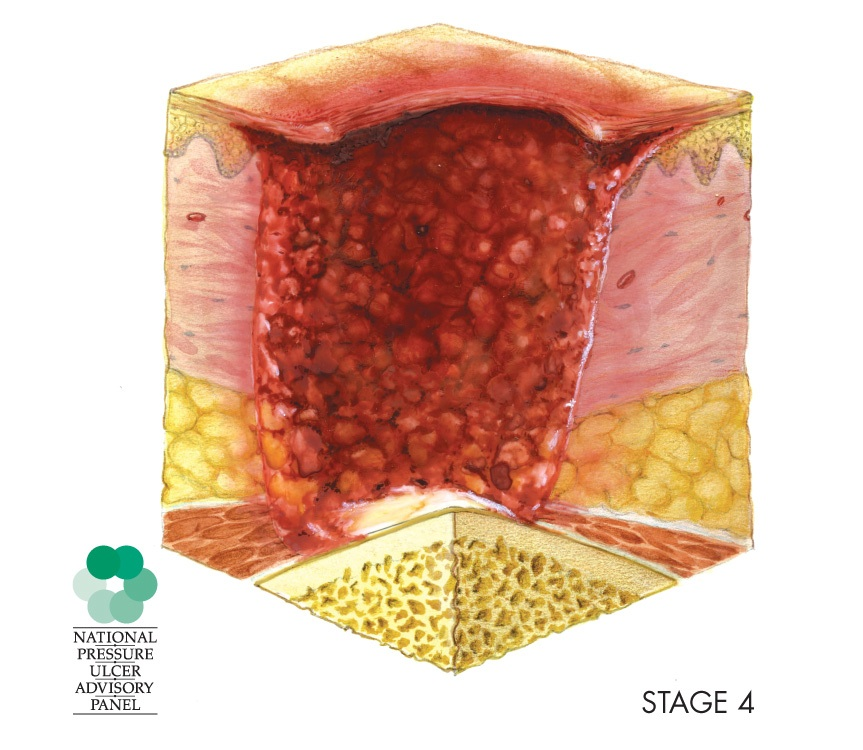
\includegraphics[width=0.33\textwidth]{../latex/assets/npuap/stage4.png}}
						\subfloat{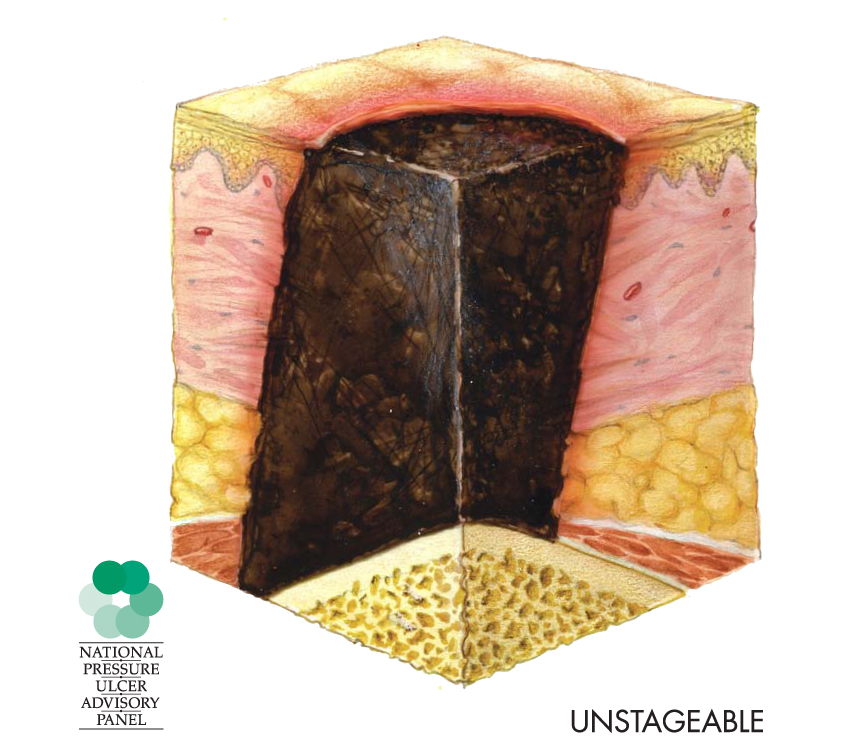
\includegraphics[width=0.33\textwidth]{../latex/assets/npuap/unstageable.png}}
						\subfloat{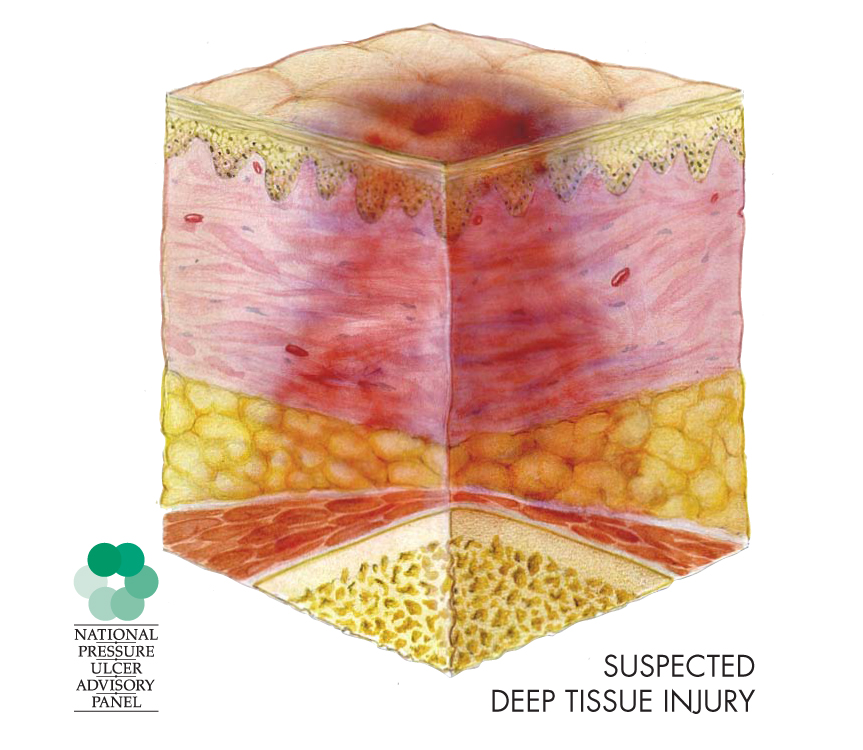
\includegraphics[width=0.33\textwidth]{../latex/assets/npuap/suspectedDTI.png}}

						\caption{\copyright\ National Pressure Ulcer Advisory Panel, used with permission.}
					\end{figure}
			\end{columns}
		\end{frame}

		\begin{frame}
			\frametitle{Introduction}
			\vspace{0.5cm}
			\begin{itemize}
				\item Earliest form of ultrasound elastography
				\item Apply manual pressure to tissue
				\begin{itemize}
					\item Measure localized deformation of tissue
				\end{itemize}
				\item Magnitude of deformation related to stiffness
				\begin{itemize}
					\item $\downarrow$ deformation $\approx$ $\uparrow$ stiffness $\approx$ $\uparrow$ damage magnitude
				\end{itemize}
			\end{itemize}

			\vspace{0.5cm}
			\begin{columns}[b]
				\column{0.5\textwidth}
					\begin{tikzpicture}[x=\textwidth,y=0.4\textwidth]
						\draw[thick, draw=ExecusharesBlack, fill=ExecusharesWhite]
						(0, 0) -- (1, 0) -- (1, 1) -- (0, 1) -- cycle;
						\draw[dashed, thick, draw=ExecusharesBlack, fill=none]
						(0.15, 0.1) -- (0.85, 0.1) -- (0.85, 1) -- (0.15, 1) -- cycle;
						\draw[thick, draw=ExecusharesBlack, fill=ExecusharesRed]
						(0.15, 1) -- (0.85, 1) -- (0.85, 1.25) -- (0.15, 1.25) -- cycle;
						\draw[ultra thick, draw=ExecusharesBlue, fill=none]
						(0.55, 0.45) -- (0.65, 0.45) -- (0.65, 0.75) -- (0.55, 0.75) -- cycle;
						\tikzset{text=ExecusharesBlue}
						\node at (0.6, 0.6) {$R_1$};
						\tikzset{text=ExecusharesBlack}
						\node at (0.5, 1.125) {US Probe};
						\tikzset{text=ExecusharesBlack}
						\node at (0.5, 0.25) {Field of View};
						\tikzset{text=ExecusharesBlack}
						\node at (0.5, -0.15) {Pre-compression image};
					\end{tikzpicture}

				\column{0.5\textwidth}
					\begin{tikzpicture}[x=\textwidth,y=0.4\textwidth]
						\draw[thick, draw=ExecusharesBlack, fill=ExecusharesWhite]
						(0, 0) -- (1, 0) -- (1, 0.8) -- (0, 0.8) -- cycle;
						\draw[dashed, thick, draw=ExecusharesBlack, fill=none]
						(0.15, 0.1) -- (0.85, 0.1) -- (0.85, 0.8) -- (0.15, 0.8) -- cycle;
						\draw[thick, draw=ExecusharesBlack, fill=ExecusharesRed]
						(0.15, 0.8) -- (0.85, 0.8) -- (0.85, 1.05) -- (0.15, 1.05) -- cycle;
						\draw[thick, draw=ExecusharesBlack, fill=ExecusharesBlue]
						(0.5, 1.1) -- (0.6, 1.2) -- (0.55, 1.2) -- (0.55, 1.25) -- (0.45, 1.25) -- (0.45, 1.2) -- (0.4, 1.2) -- cycle;
						\draw[ultra thick, draw=ExecusharesBlue, fill=none]
						(0.65, 0.45) -- (0.75, 0.45) -- (0.75, 0.65) -- (0.65, 0.65) -- cycle;
						\tikzset{text=ExecusharesBlue}
						\node at (0.7, 0.55) {$R_2$};
						\draw[ultra thick, ->, draw=ExecusharesBlue, fill=ExecusharesBlue]
						(0.55, 0.4) -- (0.65, 0.45);
						\tikzset{text=ExecusharesBlack}
						\node at (0.5, 0.925) {US Probe};
						\tikzset{text=ExecusharesBlack}
						\node at (0.5, 0.25) {Field of View};
						\node at (0.5, -0.15) {Post-compression image};
					\end{tikzpicture}
			\end{columns}
		\end{frame}

		\note{The first imaging modality I investigated was ``quasi-static ultrasound elastography'', which involves the manual manipulation of soft tissues in order to estimate deformation gradients and subsequently localized tissue strains. By comparing localized tissue strains throughout the domain, the stiffness ratio of lesions may be estimated.}